\documentclass[letter,12pt]{article}
\usepackage[paperheight=27.94cm,paperwidth=21.59cm,bindingoffset=0in,left=3cm,right=2.0cm, top=3.5cm,bottom=2.5cm, headheight=200pt, headsep=1.0\baselineskip]{geometry}
\usepackage{graphicx,lastpage}
\usepackage{upgreek}
\usepackage{censor}
\usepackage[spanish,es-tabla]{babel}
\usepackage{pdfpages}
\usepackage{tabularx}
\usepackage{graphicx}
\usepackage{adjustbox}
\usepackage{xcolor}
\usepackage{colortbl}
\usepackage{rotating}
\usepackage{multirow}
\usepackage[utf8]{inputenc}
\usepackage{float}
\usepackage{hyperref}

\renewcommand{\tablename}{Tabla}
\usepackage{fancyhdr}
\pagestyle{fancy}


%
\begin{document}
%
   \title{\Huge{Informe Laboratorio 4}}

   \author{\textbf{Sección x} \\  \\Alumno x \\ e-mail: alumno.contacto@mail.udp.cl}
          
   \date{Mayo de 2024}

   \maketitle
   
   \tableofcontents
 
  \newpage
  

\section{Descripción de actividades}
Para este laboratorio, deberá utilizar Tampermonkey y la librería CryptoJS (con SRI) para lograr obtener los mensajes que le está comunicando su informante. En esta ocasión, su informante fue más osado y se comunicó con usted a través de un sitio web abierto a todo el público https://cripto.tiiny.site/.\par
Sólo un ojo entrenado como el suyo logrará descifrar cuál es el algoritmo de cifrado utilizado y cuál es la contraseña utilizada para lograr obtener la información que está oculta.
\begin{enumerate}
    \item Desarrolle un plugin para tampermonkey que permita obtener la llave para el descifrado de los mensajes ocultos en la página web. La llave debe ser impresa por la consola de su navegador al momento de cargar el sitio web. Utilizar la siguiente estructura:
    \begin{itemize}
        \item   La llave es: KEY
    \end{itemize}
    
    \item En el mismo plugin, se debe detectar el patrón que permite identificar la cantidad de mensajes cifrados. Debe imprimir por la consola la cantidad de mensajes cifrados. Utilizar la siguiente estructura:
    Los mensajes cifrados son: NUMBER
    
    \item En el mismo plugin debe obtener cada mensaje cifrado y descifrarlo. Ambos mensajes deben ser informados por la consola (cifrado espacio descifrado) y además cada mensaje en texto plano debe ser impreso en la página web. \par
    El script desarrollado debe ser capaz de obtener toda la información del sitio web (llave, cantidad de mensajes, mensajes cifrados) sin ningún valor forzado. Para verificar el correcto funcionamiento de su script se utilizará un sitio web con otro texto y una cantidad distinta de mensajes cifrados. Deberá indicar la url donde se podrá descargar su script.\par
    Un ejemplo de lo que se debe visualizar en la consola, al ejecutar automáticamente el script, es lo siguiente:

    \begin{figure}[H]
        \centering
        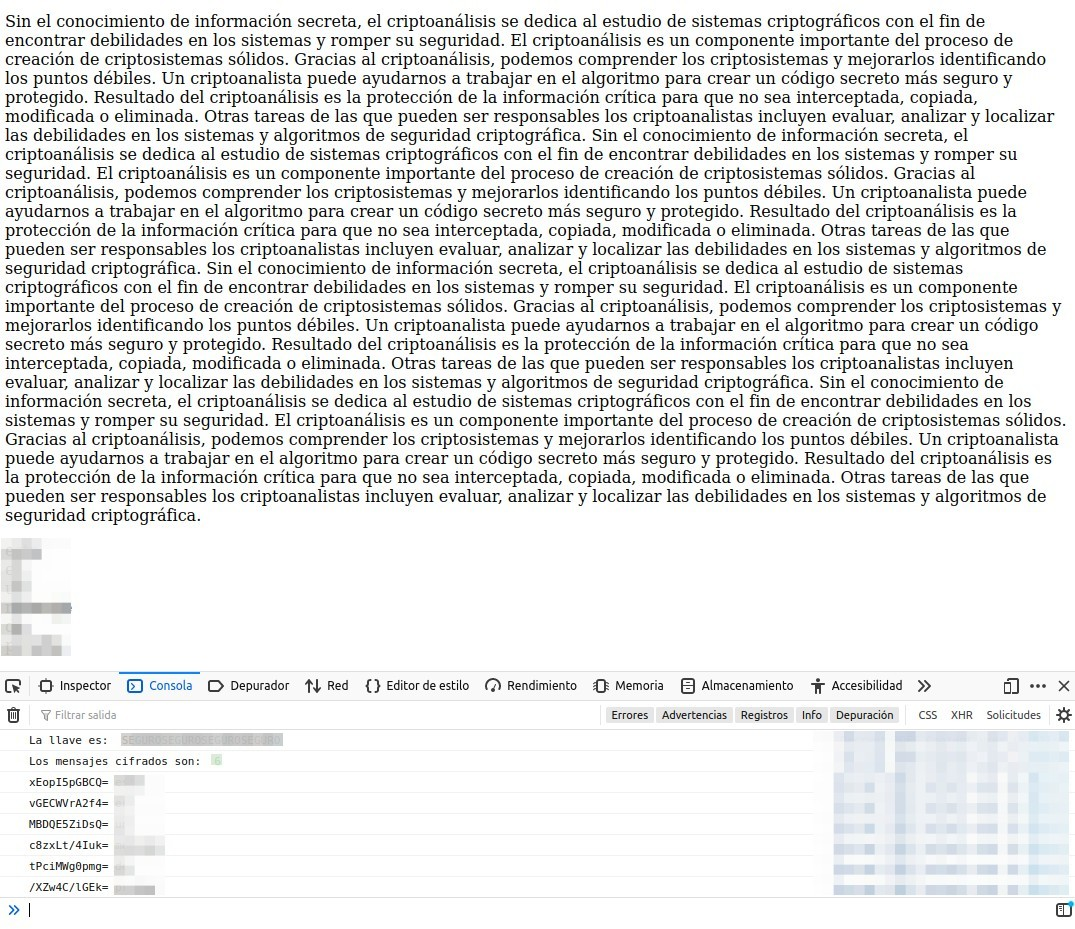
\includegraphics[width=16cm]{Desarrollo/ejemplo.jpg}
        \label{fig:ejemplo}
    \end{figure}

\end{enumerate}

\section{Desarrollo (Parte 1)}
\subsection{Detecta el cifrado utilizado por el informante}
\subsection{Logra que el script solo se gatille en el sitio usado por el informante}
\subsection{Define función que obtiene automáticamente el password del documento}
\subsection{Muestra la llave por consola}

\section{Desarrollo (Parte 2)}

\subsection{Reconoce automáticamente la cantidad de mensajes cifrados}

\subsection{Muestra la cantidad de mensajes por consola}

\section{Desarrollo (Parte 3)}

\subsection{Importa la librería cryptoJS}

\subsection{Utiliza SRI en la librería CryptoJS}

\subsection{Repercusiones de SRI inválido}

\subsection{Logra decifrar uno de los mensajes}

\subsection{Imprime todos los mensajes por consola}

\subsection{Muestra los mensajes en texto plano en el sitio web}

\subsection{El script logra funcionar con otro texto y otra cantidad de mensajes}

\subsection{Indica url al código .js implementado para su validación}

\section*{Conclusiones y comentarios}

\subsection*{Issues}

\end{document}
